%&tex
\chapter{Disentanglement of Shape and Appearance}\label{sec:disentangling}
	Disentangled representations of object shape and appearance allow to alter both properties individually to synthesize new images. The ability to flexibly control the generator allows, for instance, to change the pose of a person or their clothing. In contrast to previous work \cite{esser18, denton17disvideo, ma17poseguided, ma17disperson, debem18dgpose, jakab18},
	we achieve this ability without requiring supervision \textit{and} using a flexible part-based model instead of a holistic representation. This allows to explicitly control the parts of an object that are to be altered. We quantitatively compare against \emph{supervised} state-of-the-art disentangled synthesis of human figures. Also we qualitatively evaluate our model on unsupervised synthesis of still images, video-to-video translation, and local editing for appearance transfer.
	\todo{incorporate following to make more expressive}
	% In this section we provide evidence that the proposed object factorization into local parts with shape and appearance components is indeed achieved by our model.
	% As is common for supervised disentangling methods, to evaluate the disentanglement of internal factors, we use the generated images to access the internal representation.
	% The global disentanglement of shape and appearance is tested on the task of conditional image generation and video-to-video translation, while the local part-wise disentanglement is tested on the task of part appearance transfer. \\
	% \textbf{Conditional Image Generation}
	% In a disentangled representation of object shape and appearance it should be possible to generate from the same shape with different appearances and vice versa.
	% In our model we can choose the shape or appearance conditioning by providing images as input to the shape or the appearance stream.

\section{Disentangling Pose and Appearance}\label{sec:poseandappearance}
		% POSE APPEARANCE SWAP
		\begin{figure}[htp]
			\centering
			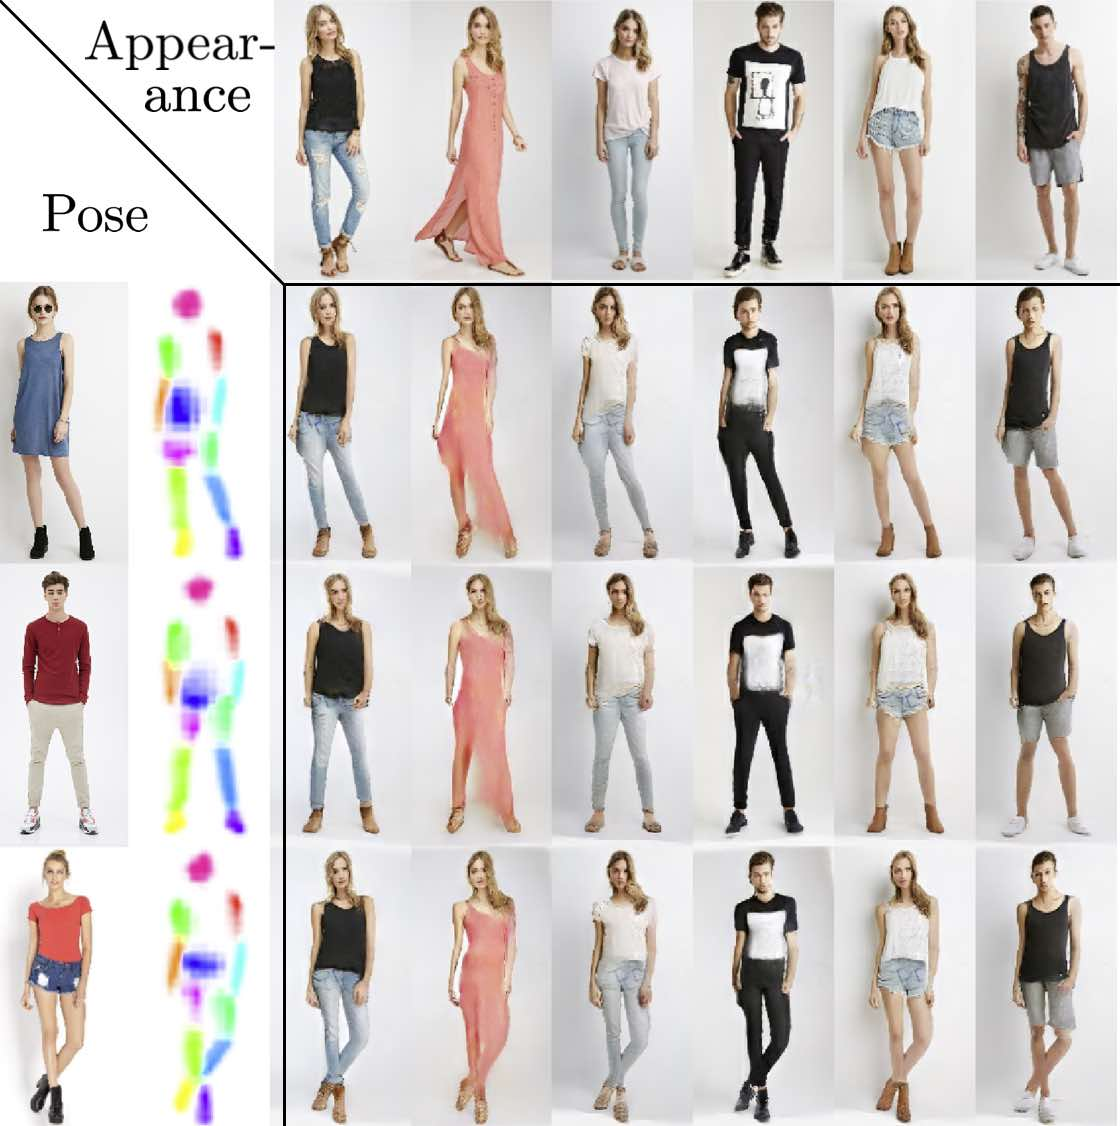
\includegraphics[trim={0cm 0cm 0cm 0cm},clip, width=.5\linewidth]{fig/factor/swappy}
			\caption{Transferring shape and appearance on Deep Fashion. Without annotation the model estimates shape, 2nd column. Target appearance is extracted from images in top row to synthesize images. Note that we trained without image pairs only using synthetic transformations.
			%for training we had no image pairs but only synthetic transformations.
			%without being explicitly trained for this task.
			All images are from the test set.}
			\label{fig:allswaps}
		\end{figure}

		On Deep Fashion \cite{liu16deepfashion, liu16deepfashionwild}, a benchmark dataset for supervised disentangling methods, the task is to separate person ID (appearance) from body pose (shape) and then synthesize new images for previously unseen persons from the test set in eight different poses. We randomly sample the target pose and appearance conditioning from the test set. Fig. \ref{fig:allswaps} shows qualitative results.
		\todo{incorporate note}
		\note{We compare the disentangling performance quantitatively against a supervised method, namely the variational U-Net \cite{Esser:2018ue}. We evaluate on the DeepFashion dataset, a standard benchmark dataset for supervised disentangling methods. In this dataset appearance is defined by a persons ID and shape by the pose of the person. For each ID in the test set, we condition the image generation on 8 different poses which are chosen randomly from the test set. Both VU-Net and our model are conditioned on the exactly the same pose-ID image pairs.
		We quantitatively compare against supervised state-of-the-art disentangling \cite{esser18} by evaluating \emph{i)} invariance of appearance against variation in shape by the re-identification error and \emph{ii)} invariance of shape against variation in appearance by the distance in pose between generated and pose target image.}

		\begin{tcolorbox}
			\textbf{Deep Fashion} \cite{liu16deepfashion, liu16deepfashionwild} consists of ca. 53k in-shop clothes images in high-resolution of $256 \times 256$. We selected the images which are showing a full body (all keypoints visible, measured with the pose estimator by \cite{cao17affinityfield}) as full visibilty of the object is an assumption to the model and used the provided train-test split. For comparison with Esser \etal \cite{esser18} we used their published code.
		\end{tcolorbox}

	\subsection{Person Re-Identification}

		Person re-identification (ReID) is a research field on its own (overview in \eg \cite{almazan18reidtowards, bedagkar14reidtrends}), the goal being to learn a similarity metric for a persons appearance, invariant to a persons posture and the image viewpoint.
		% zheng16reidcnn
		The key applications are automated person tracking and surveillance \cite{zheng16reidfuture}.
		For our purposes, we will treat a ReID algorithm as a metric for measuring the preservation of appearance as well as the invariance to shape on our generated images.
		For this, we fine-tune an ImageNet-pretrained \cite{russakovsky15imagenet} Inception-Net \cite{szegedy15inception} with a ReID algorithm \cite{xiao17reidjoint} via a triplet loss \cite{hermans17reidtriplet} to the Deep Fashion training set.
		On the generated images we report the standard metrics for ReID, mean average precision (mAP) and rank-1, -5, and -10 accuracy.
		\todo{explain these metrics}
		% These metrics express
		% In single-image ReID the task is to
		% many-image ReID
		% ReID means ranking. rank-1 is the ratio of correct finding by the first entry. rank-n ratio of correct samples that are within first n entries in ranking. mean average precision is the average over
		The first question we ask, is, if the appearance encoding is stable to variations in pose, hence invariant to pose (shape). Each ID from the test set is generated in 8 different poses. The task for the ReID algorithm is now to rank the similarity of these pose-changed yet same-appearance generations.
		Although our approach is unsupervised, it is competitive compared to the supervised VU-Net \cite{esser18} as shown in Tab. \ref{tab:reid}. The high chance of reidentifying a persons appearance in a different shape (rank-1 accuracy) shows that the appearance is invariant against variation in shape (pose) for both methods.
 		To visualize the closeness of the same-ID generations in the ReID-embedding the show a t-SNE plot in Fig.~\ref{fig:tsne}.

		\begin{table}[htp]
			\centering
			\caption{Mean average precision (mAP) and rank-n accuracy for person re-identification on synthesized images after performing shape/appearance swap. Input images from Deep Fashion test set. Note \cite{esser18} is supervised \wrt shape.}
			\label{tab:reid}
			\begin{tabular}{l|cccr}
				\hline
				& mAP & rank-1 & rank-5 & rank-10 \\ \hline
				VU-Net \cite{esser18} & 88.7\% & 87.5\% & {98.7}\% & {99.5}\% \\
				Ours & {90.3}\% & {89.4}\% &{98.2}\% & {99.2}\% \\ \hline
			\end{tabular}
		\end{table}

		% TSNE
		\begin{figure}[htp]
			\centering
			\begin{subfigure}{0.49\linewidth}
			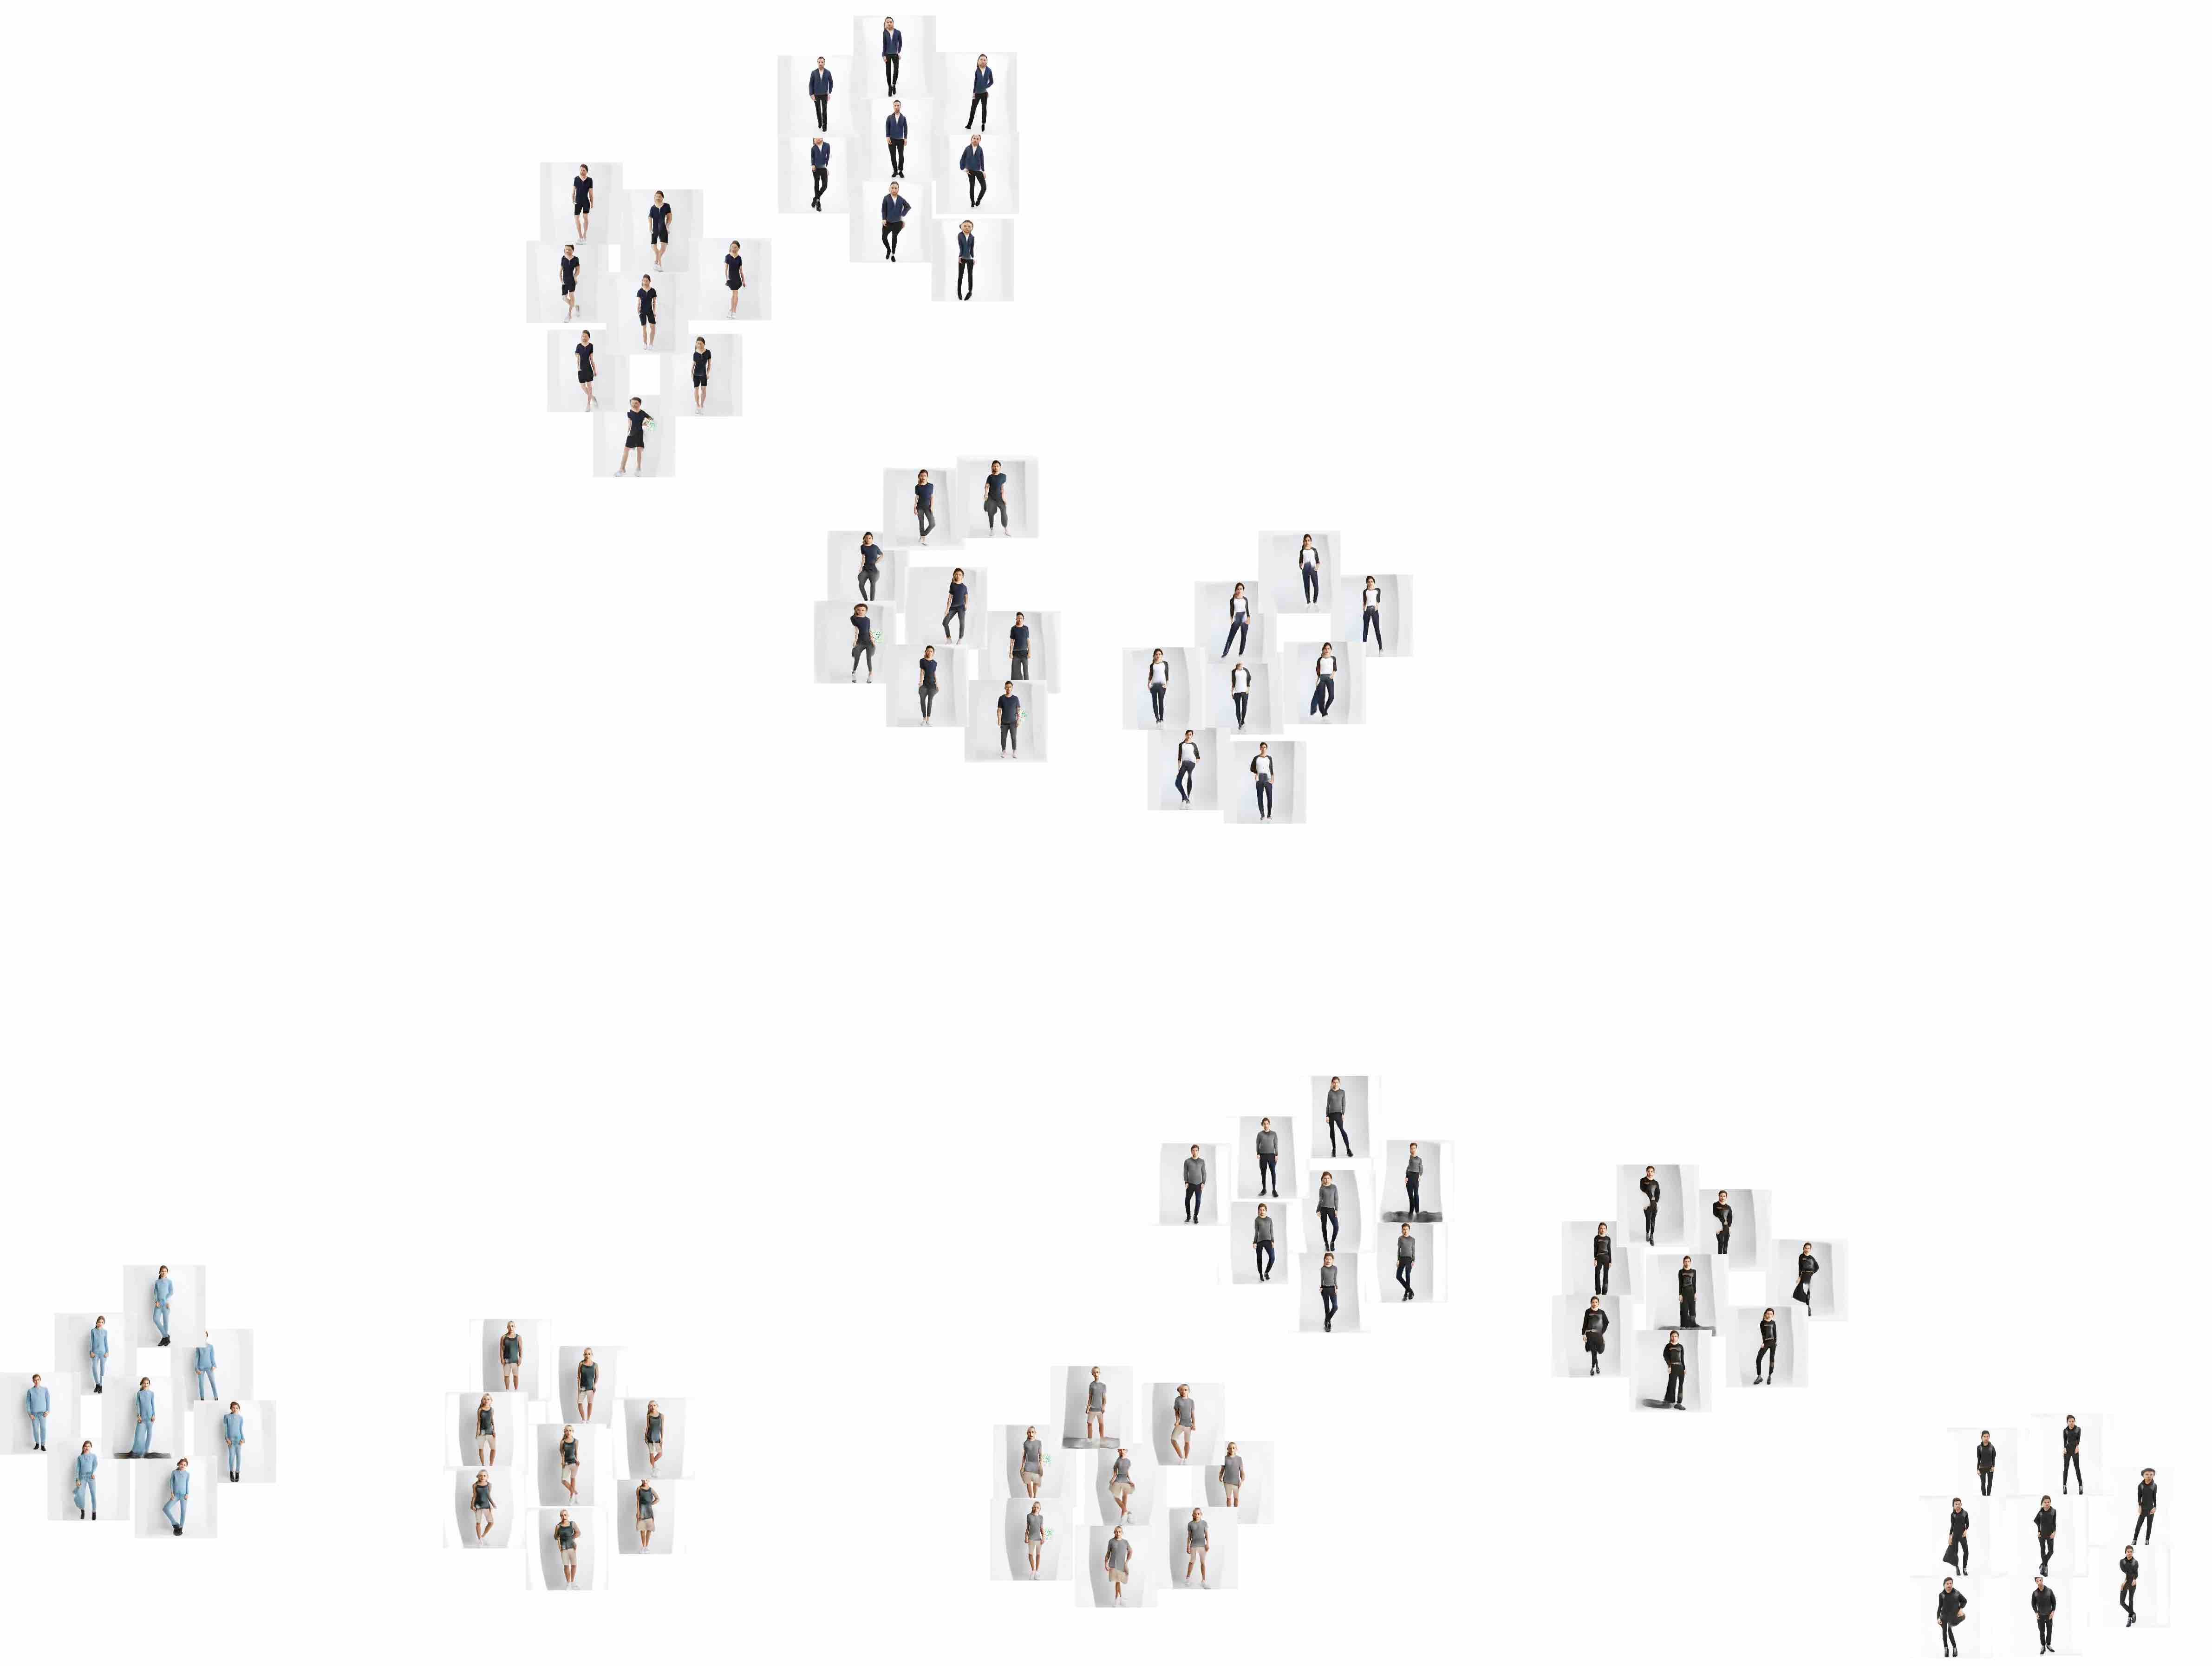
\includegraphics[trim={0cm 0cm 0cm 0cm},clip, width=1.0\linewidth]{fig/factor/tsne_img}
			\end{subfigure}
			\begin{subfigure}{0.49\linewidth}
			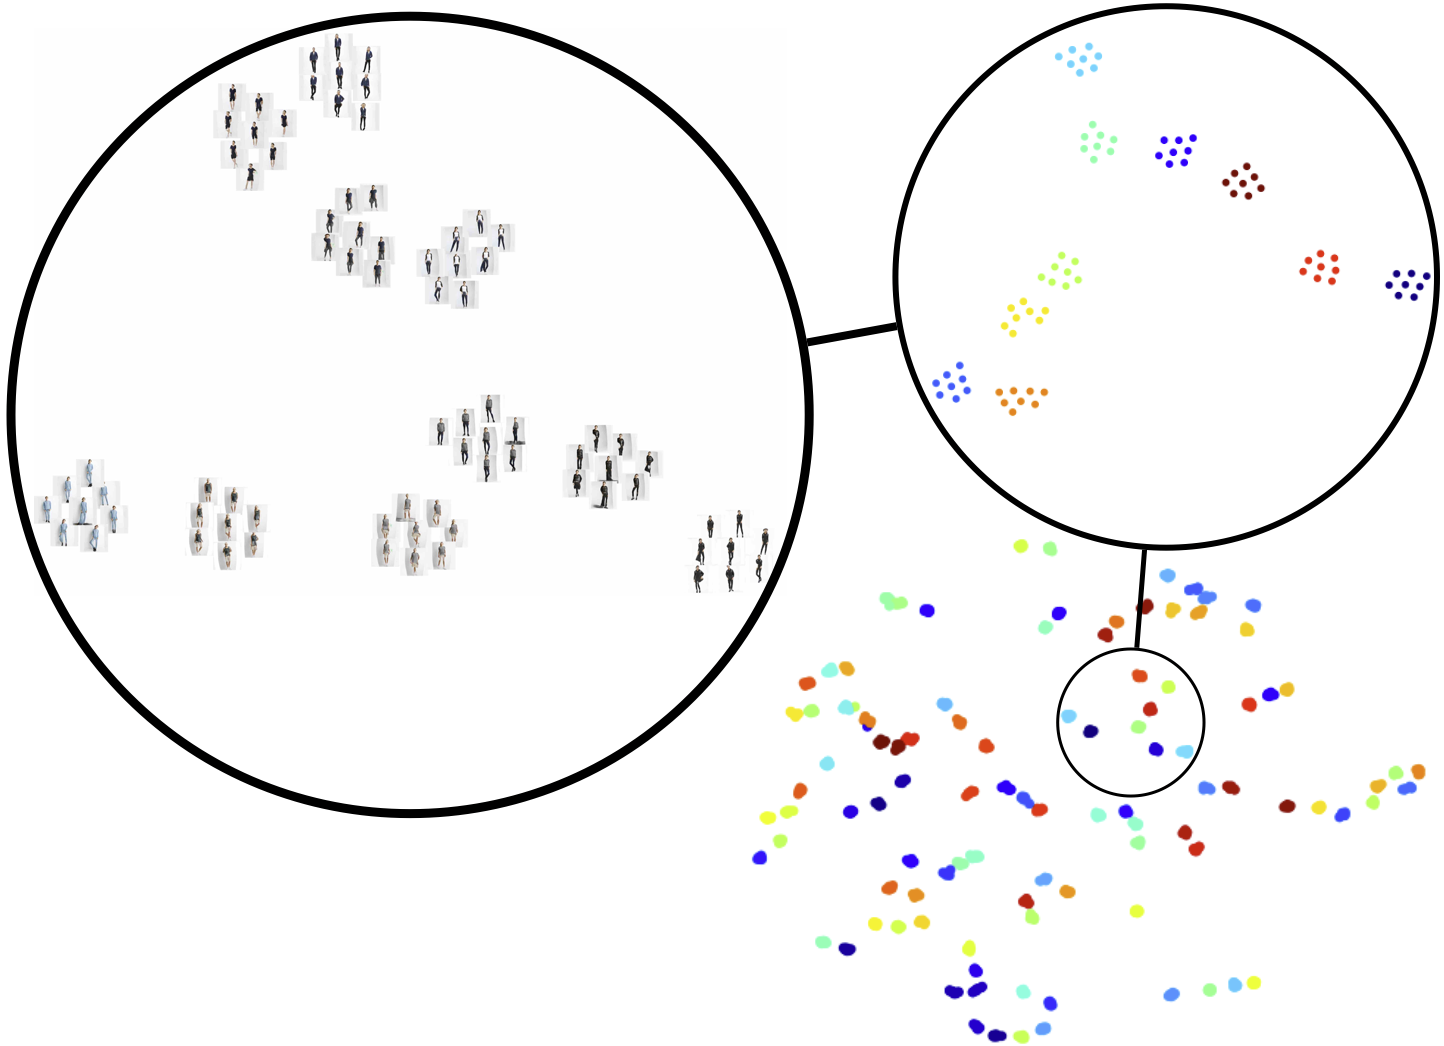
\includegraphics[trim={0cm 0cm 0cm 0cm},clip, width=1.0\linewidth]{fig/factor/tsne_bubble}
			\end{subfigure}
			% \begin{subfigure}{0.49\linewidth}
				% % \begin{subfigure}{0.49\linewidth}
				% 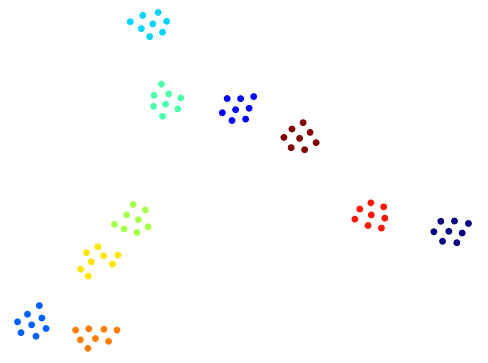
\includegraphics[trim={0cm 0cm 0cm 0cm},clip, width=1.0\linewidth]{fig/factor/tsne10}
				% \end{subfigure}\begin{subfigure}{0.49\linewidth}
				% 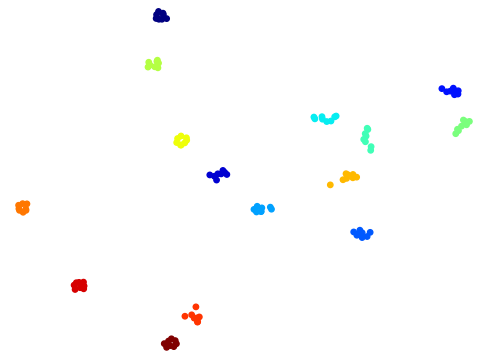
\includegraphics[trim={0cm 0cm 0cm 0cm},clip, width=1.0\linewidth]{fig/factor/tsne15}
				% \end{subfigure}
				% \begin{subfigure}{0.49\linewidth}
				% 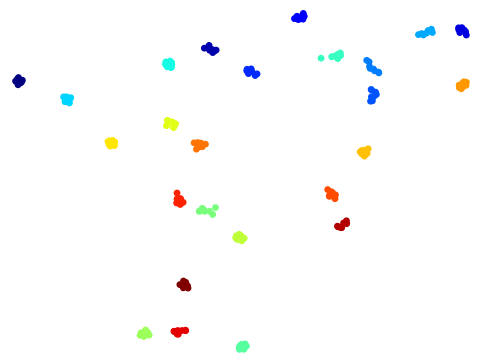
\includegraphics[trim={0cm 0cm 0cm 0cm},clip, width=1.0\linewidth]{fig/factor/tsne20}
				% \end{subfigure}
				% \begin{subfigure}{0.49\linewidth}
				% 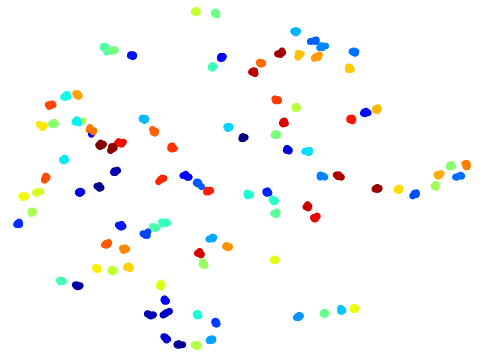
\includegraphics[trim={0cm 0cm 0cm 0cm},clip, width=1.0\linewidth]{fig/factor/tsne100}
				% \end{subfigure}
			% \end{subfigure}
			\caption{Visualization of feature distribution for generated person IDs. (Right) t-SNE (perplexity 16) of 10 generated IDs, (left) color-coded t-SNE (perplexity 12) for 10, 15, 20 and 100 IDs. Each ID has 8 samples. The different IDs are clearly separable, despite variation in pose: Hence, generated appearance is invariant to pose.}
			\label{fig:tsne}
		\end{figure}

		The second question one could ask is, if appearance is preserved, \ie if the ReID algorithm is able to reidentify the groundtruth appearance image from the generation. Results for this are shown in Tab.~\ref{tab:reiddirect}. The result depends strongly on whether the algorithm had been fine-tuned to the DeepFashion image distribution or the DeepFashion and the synthesized image distribution. The stark difference can be explained by the difference in the feature distribution: high-frequency details (such as patterns and texture of clothing), are not synthesized correctly, as the model is trained by a reconstruction objective which will blurr these high frequencies. On the other hand, the adversarial objective will encourage \textit{some} high frequencies, but not necessarily the ones from the initial appearance conditioning. The ReID algorithm, if not additionally adjusted to this, will pay attention to those details and subsequently fail.
		unambiguous function between generations and groundtruth can be found.

		\begin{table}[htp]
			\centering
			\caption{Mean average precision (mAP) and rank-n accuracy for person re-identification from synthesized to ground truth appearance images after performing shape/appearance swap. When only fine-tuning the ReID algorithm on DeepFashion, results are much worse that when also adjusting to the synthesized images.}
			\label{tab:reiddirect}
			\begin{tabular}{l|cccr}
				\hline
				Fine-tune to: & mAP & rank-1 & rank-5 & rank-10 \\ \hline
				% VU-Net \cite{esser18} & 88.7\% & 87.5\% & {98.7}\% & {99.5}\% \\
				DeepFashion & {17.2}\% & {25.4}\% &{48.8}\% & {60.4}\% \\
				DeepFashion and Synthesized Images& {75.0}\% & {73.8}\% &{89.5}\% & {92.5}\% \\ \hline
			\end{tabular}
		\end{table}



		\subsection{Pose Estimation}
		% \begin{figure}[htp]
			% \centering
			% \begin{subfigure}{0.49\linewidth}
			% 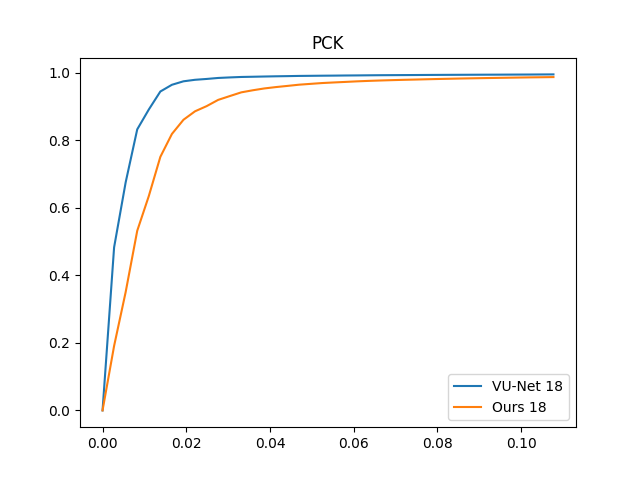
\includegraphics[trim={0cm 0cm 0cm 0cm},clip, width=1.0\linewidth]{fig/pck18}
			% \end{subfigure}
			% \begin{subfigure}{0.49\linewidth}
			% 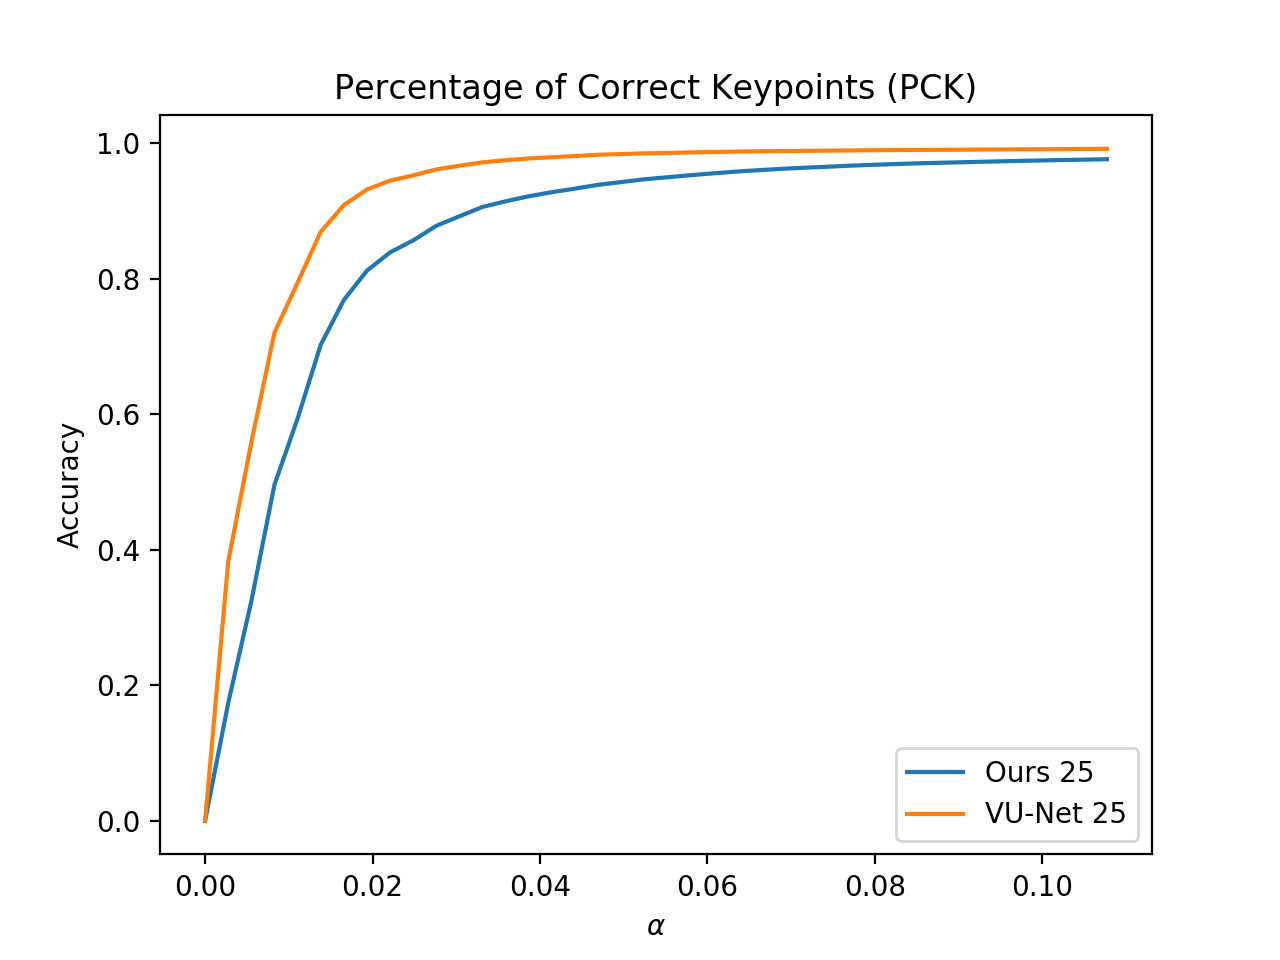
\includegraphics[trim={0cm 0cm 0cm 0cm},clip, width=0.7\linewidth]{fig/factor/pck25}
			% \end{subfigure}
			% \caption{PCK Curve for VU-Net \cite{esser18} and Ours for re-estimating pose with a 25 keypoint human pose detector.}
			% \label{fig:pckcurve}
		% \end{figure}

		\begin{table}[htp]
			\centering
			\caption{Percentage of Correct Keypoints (PCK) for pose estimation on shape/appearance swapped generations.\;$\alpha$ is pixel distance divided by image diagonal. Note that \cite{esser18} serves as upper bound, as it uses the groundtruth shape estimates.}
			%shape supervision.}
			\label{tab:pose}
			\begin{tabular}{l|cccr}
				\hline
				$\alpha$ & $2.5\%$ &  $5\%$ & $7.5\%$ & $10\%$ \\ \hline
				VU-Net \cite{esser18} & {95.2}\% & {98.4}\% & {98.9}\% & {99.1}\% \\
				Ours & 85.6\% & 94.2\% &96.5\% & 97.4\% \\ \hline
			\end{tabular}
		\end{table}


		To evaluate shape, we extract keypoints using a pose estimator \cite{cao17affinityfield}. Tab. \ref{tab:pose} reports the difference between generated and pose target in percentage of correct keypoints (PCK).
		% , Fig. \ref{fig:pckcurve} shows the comparison of PCK curves.
		As would be expected, VU-Net performs better, since it is trained with exactly the keypoints of \cite{cao17affinityfield}. Nevertheless, our approach achieves an impressive PCK without supervision underlining value of the embedding of object shape and the disentanglement of appearance and shape. Despite random variation in appearance the shape does not change, this can also be directly observed from the conditioned generations in Fig.~\ref{fig:allswaps}.



\section{Disentangling in a Temporal Sequence}\label{sec:videotovideo}

	\begin{figure}[htp]
		\centering
		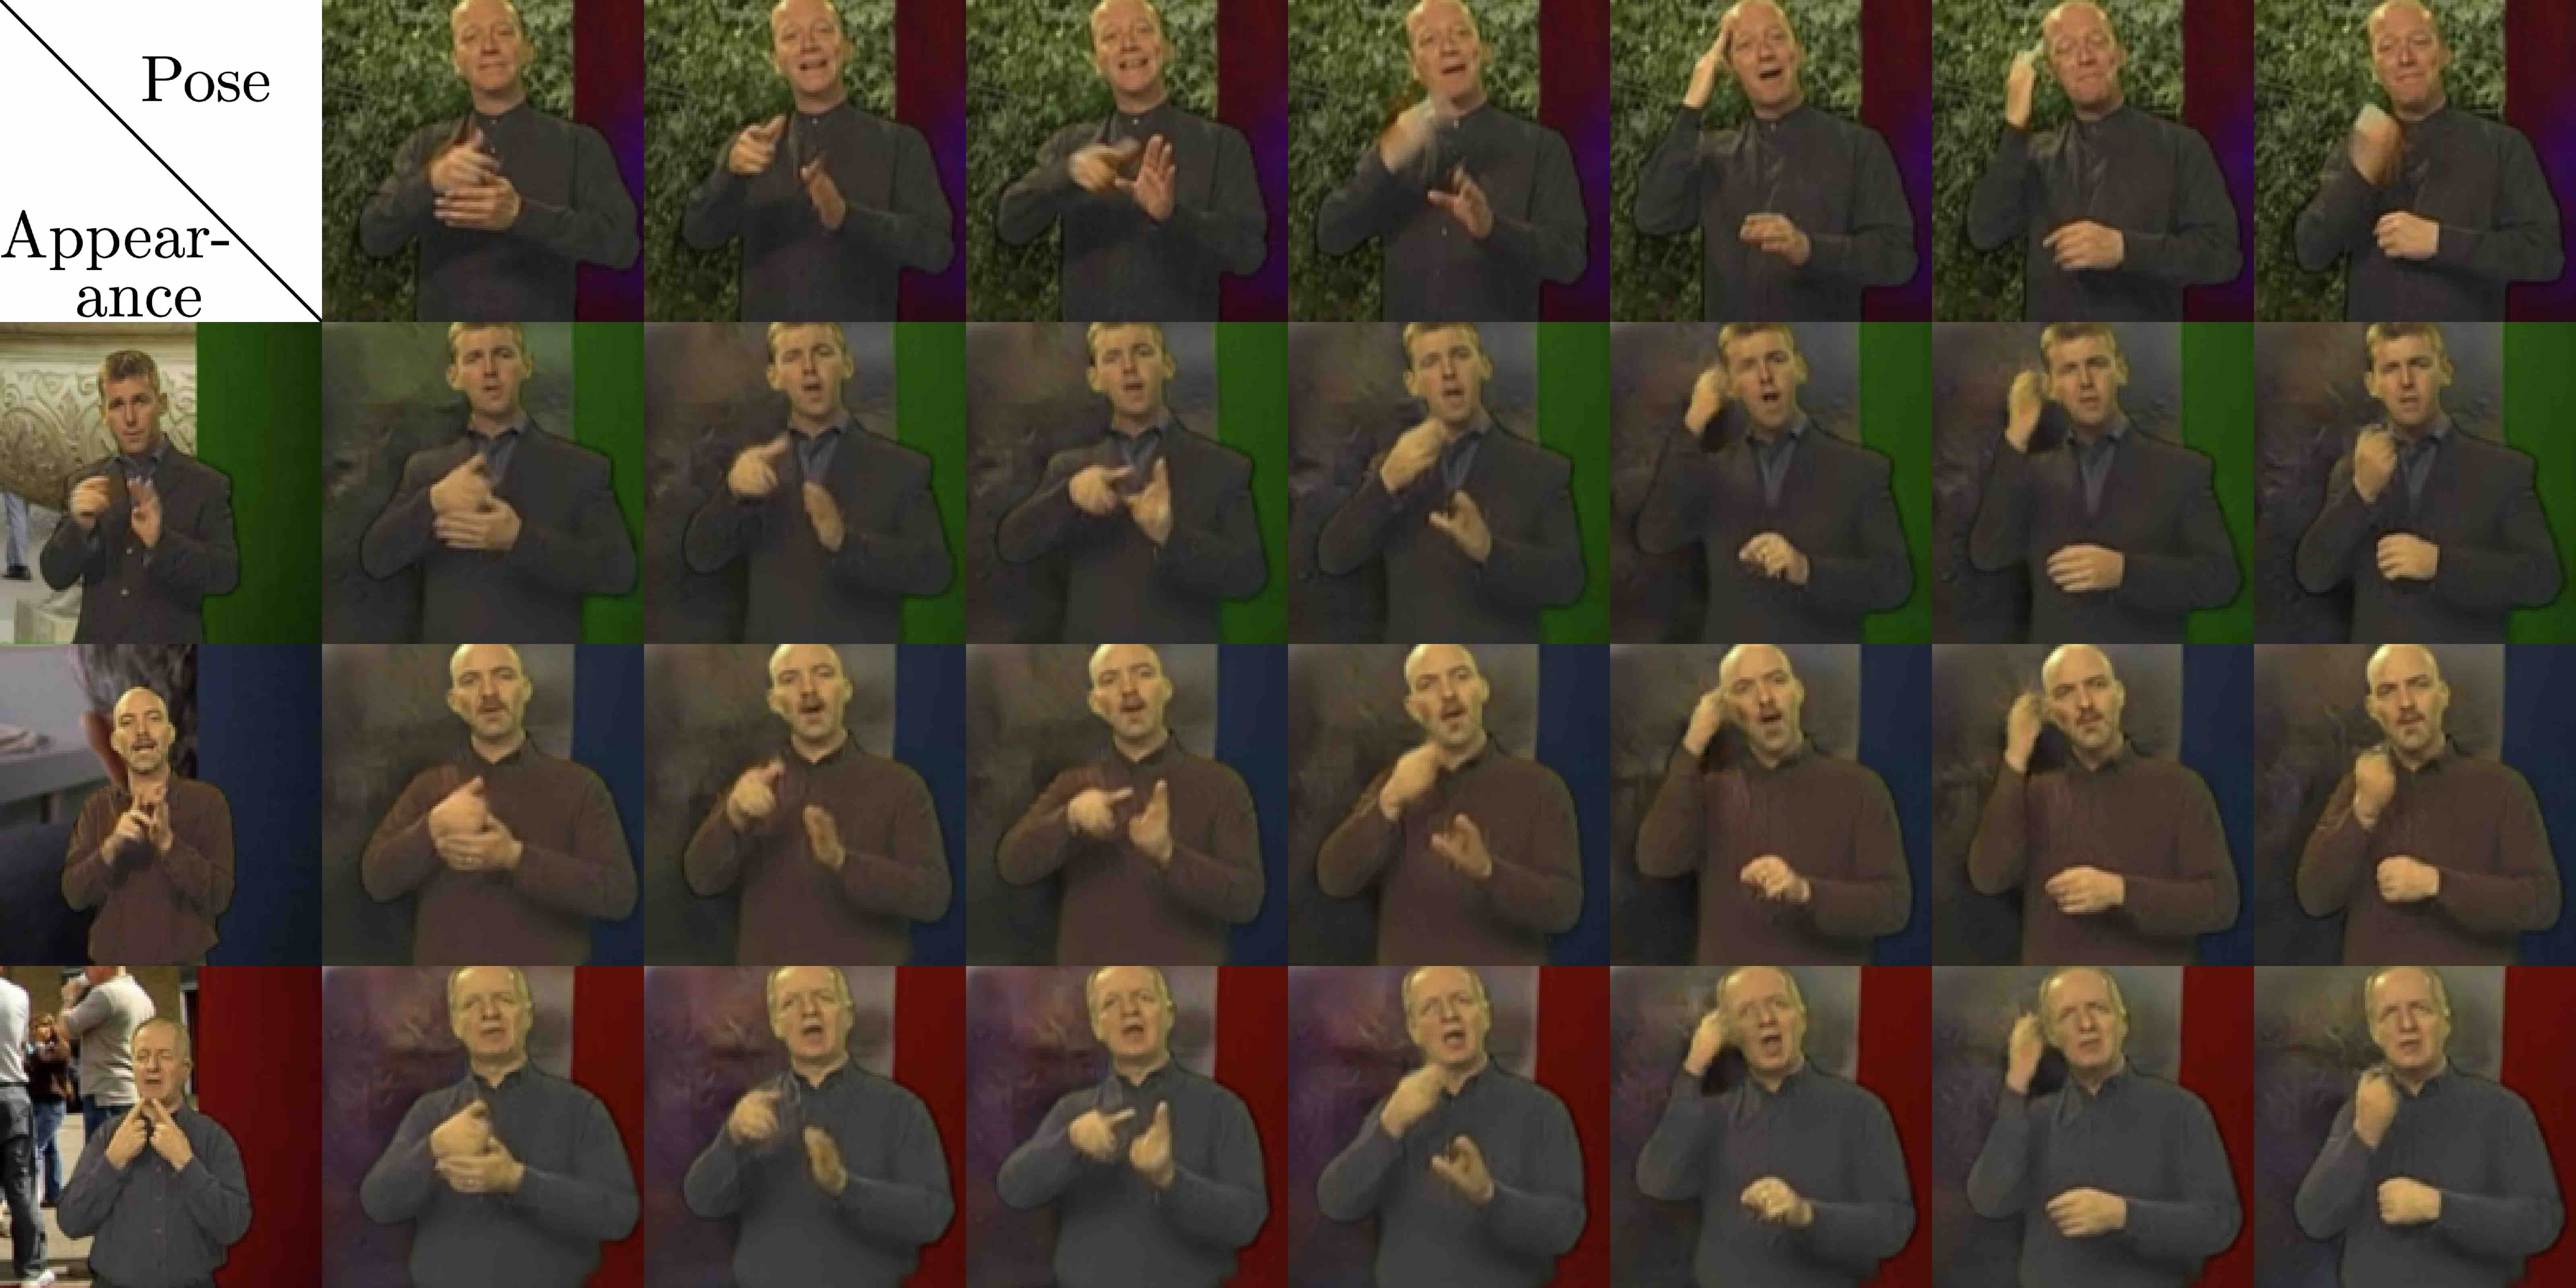
\includegraphics[trim={0cm 0cm 0cm 0cm},clip, width=1.\linewidth]{fig/factor/bbc_arrange}
		\caption{Generation results for conditioning appearances (top row) on pose (bottom, rightmost) on BBCPose.
		% The target appearances are from the train set, while the target pose is from the test set.
		Note that even fine-grained details in shape, such as fingers and facial expression are accurately captured.}
		\label{fig:bbcthumb}
	\end{figure}



	Conditional image generation can also be extended to the task of {video-to-video translation}. The two conditioning images can be frames from different videos. One frame is acting as the appearance conditioning and the other as shape conditioning. By generating each frame conditioned on the shape and appearance from two videos, one effectively transfers the appearance of one video to the shape of the other on a frame-to-frame level.
	We evaluate this frame-to-frame video translation on the BBCPose dataset. The datasets videos of sign language present a delicate and complex articulation of arms and hands. We condition on appearance from videos in the training set and on shape from videos in the test set. A sample for generated frames is shown in Fig. \ref{fig:bbcthumb}, for the complete videos please refer to the supplementary.
	We want to point out two features of the model here: Firstly, despite no use of smoothing or interpolation between frames the generated sequence is smooth in the temporal domain. This is enabled by a temporally consistent part assignment which is stable across articulation.
	Secondly, the training on the natural spatial transforms in video data enables the model to encapsulate realistic transitions such as out-of-plane rotation and complex 3D articulation of \eg hands and even fingers (note the correct translation of the thumbs position in Fig. \ref{fig:bbcthumb}). \\
	% \begin{itemize}
		% \item video-translation on BBCPose (frame-to-frame shape-appearance swap)
			% \begin{itemize}
				% \item $\Rightarrow$ shows realistic 3D transitions can be encapsulated in model by explicitly training on them (video data)
				% \item NO additional smoothing for frame-to-frame translation
					% $\Rightarrow$ latent space is consistent and smooth across time
			% \end{itemize}
	% \end{itemize}

\section{Part-wise Disentanglement}\label{sec:partwise}
	The second type of disentanglement we approach is to factorize the object into local parts. Obviously, object parts are in general not disentangled factors in a sense that they have an independent probability distribution\todo{ref to equation independence in beginning}. Since the parts are geometrically connected, in their spatial layout they are conditioned on each other. For example, you cannot move your head arbitrarily far away from your shoulders. Still, there is a local freedom and modularity - especially in appearance features - that renders a local factorization efficient. As an illustration, the color of the shoes you wear need only be mildly correlated with your hair color.
	We show that the model disentangles these local modes of variation for a persons appearance (Sec.~\ref{sec:partappearance}) and shape (Sec.~\ref{sec:partshape}).

	\subsection{Part-wise Appearance Transfer}\label{sec:partappearance}
	% PART SWAPS
	\begin{figure}[htp]
		\begin{subfigure}{0.49\linewidth}
		\centering
		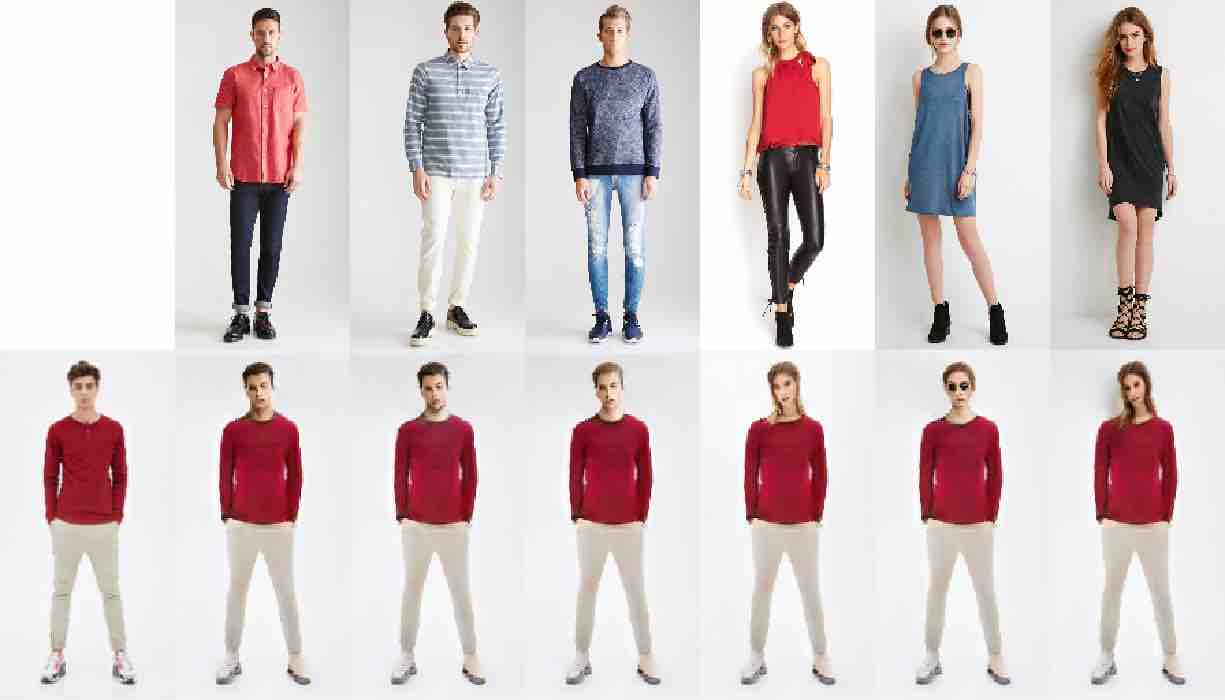
\includegraphics[trim={0cm 0cm 0cm 0cm},clip, width=1.\linewidth]{fig/factor/part6_01}\caption{}
		\label{fig:part3_00}
		\end{subfigure}
		\begin{subfigure}{0.49\linewidth}
		\centering
		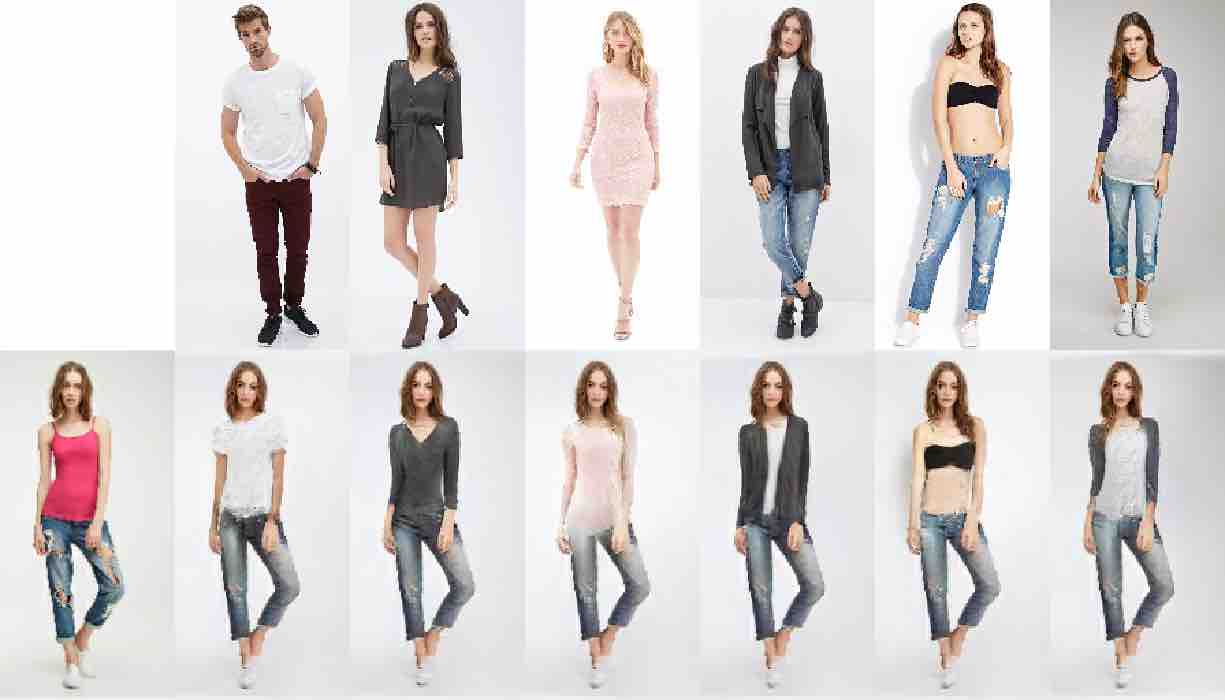
\includegraphics[trim={0cm 0cm 0cm 0cm},clip, width=1.\linewidth]{fig/factor/part6_10}\caption{}
		\label{fig:part3_11}
		\end{subfigure}
		\begin{subfigure}{0.49\linewidth}
		\centering
		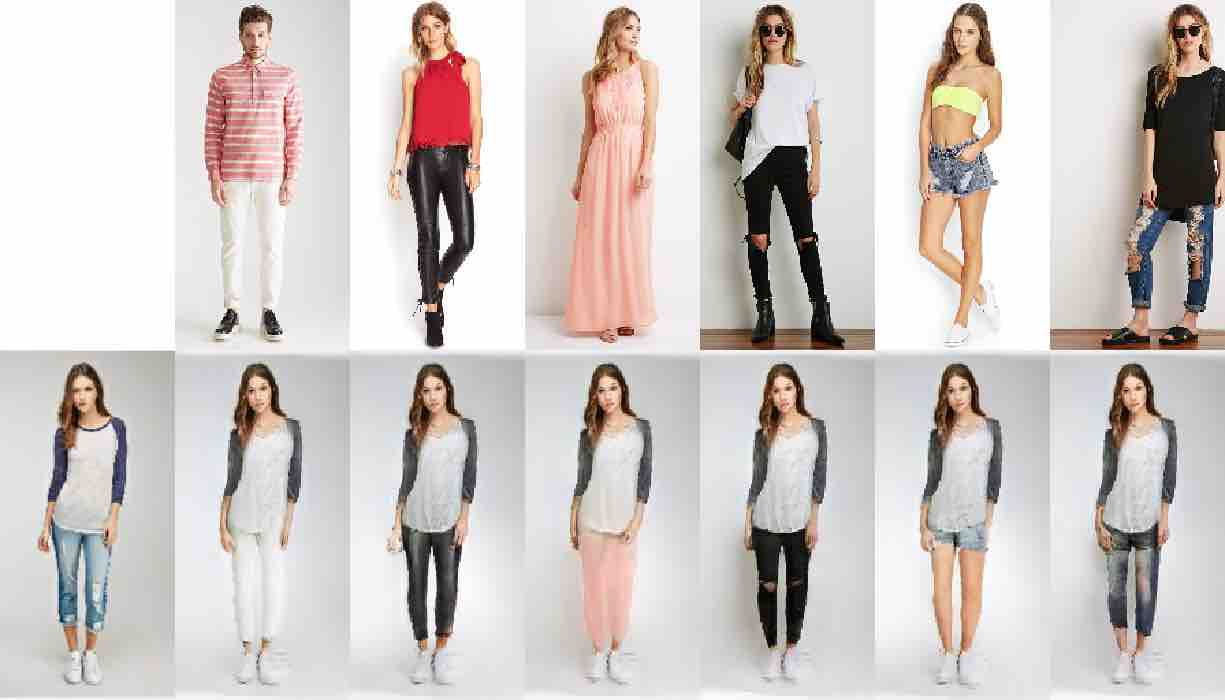
\includegraphics[trim={0cm 0cm 0cm 0cm},clip, width=1.\linewidth]{fig/factor/part6_21}\caption{}
		\label{fig:part3_21}
		\end{subfigure}
		\begin{subfigure}{0.49\linewidth}
		\centering
		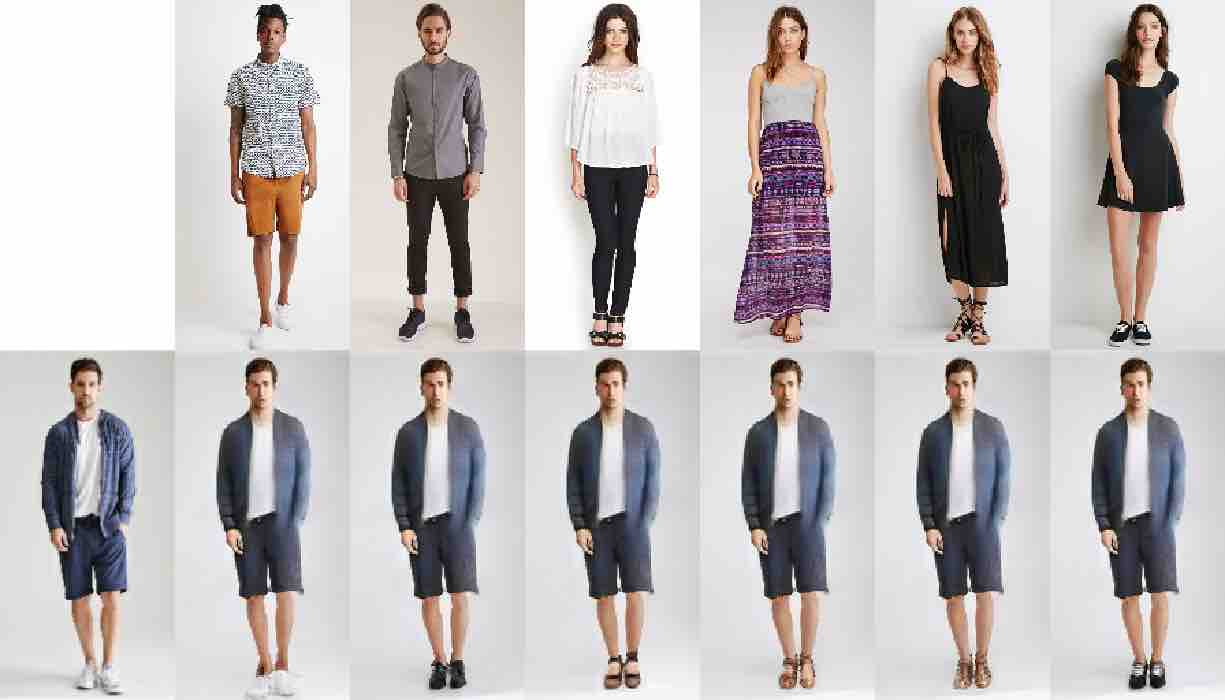
\includegraphics[trim={0cm 0cm 0cm 0cm},clip, width=1.\linewidth]{fig/factor/part6_30}\caption{}
		\label{fig:part3_30}
		\end{subfigure}
		\caption{Swapping part appearance on Deep Fashion. Appearances can be exchanged for parts individually and without altering shape. We show part-wise swaps for (a) head (b) torso (c) legs, (d) shoes. All images are from the test set.}
		\label{fig:partswaps}
	\end{figure}

	The local modelling of parts allows for a part-wise transfer of appearance. In Fig. \ref{fig:partswaps} we show the image generation conditioned on a target shape and appearance from a single image, but for several parts the appearance is transferred from another image. This shows a possible application as a virtual try-on generation, as in \cite{han17viton}.
	% \begin{itemize}
		% \item local part-appearance swaps (Fig. \ref{fig:partswaps})
			% \begin{itemize}
				% \item $\Rightarrow$ possible application, shows appearance disentangles also on part-level
			% \end{itemize}
	% \end{itemize}
	% $\Rightarrow$ Factorization achieved, utility for downstream tasks

	\subsection{Part-wise Shape Changes}\label{sec:partshape}
	One can also change the position of individual parts in the shape conditioning, which leads to generations as shown in Fig.~\ref{fig:movekp}. One can observe that the other non-moved parts shapes also lead to stationary parts in the generation, indicating that these parts are spatially disentangled. In the unnatural (never seen in data) regime \eg if the head is to far from the shoulders, the model still hallucinates a head next to the body - similar to supervised results~\cite{debem18dgpose}.

	\begin{figure}[htp]
		\centering
		\begin{subfigure}{1.\linewidth}
			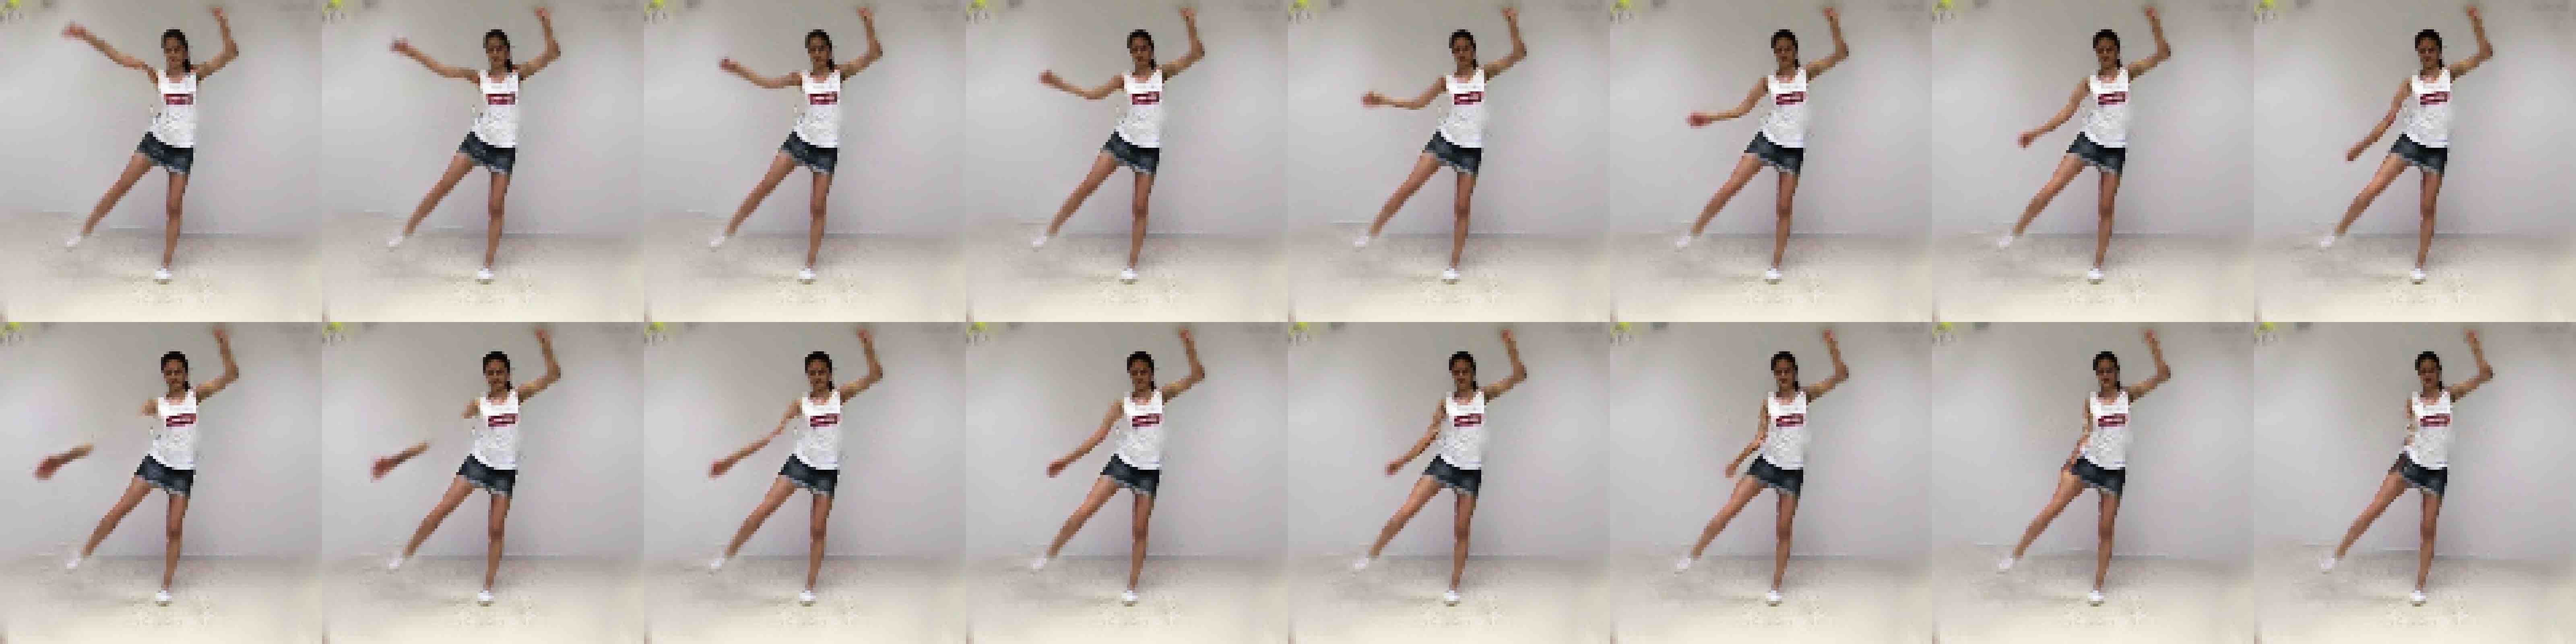
\includegraphics[trim={0cm 0cm 0cm 0cm},clip, width=1.0\linewidth]{fig/factor/8arm}\caption{}
		\end{subfigure}
		\begin{subfigure}{1.\linewidth}
			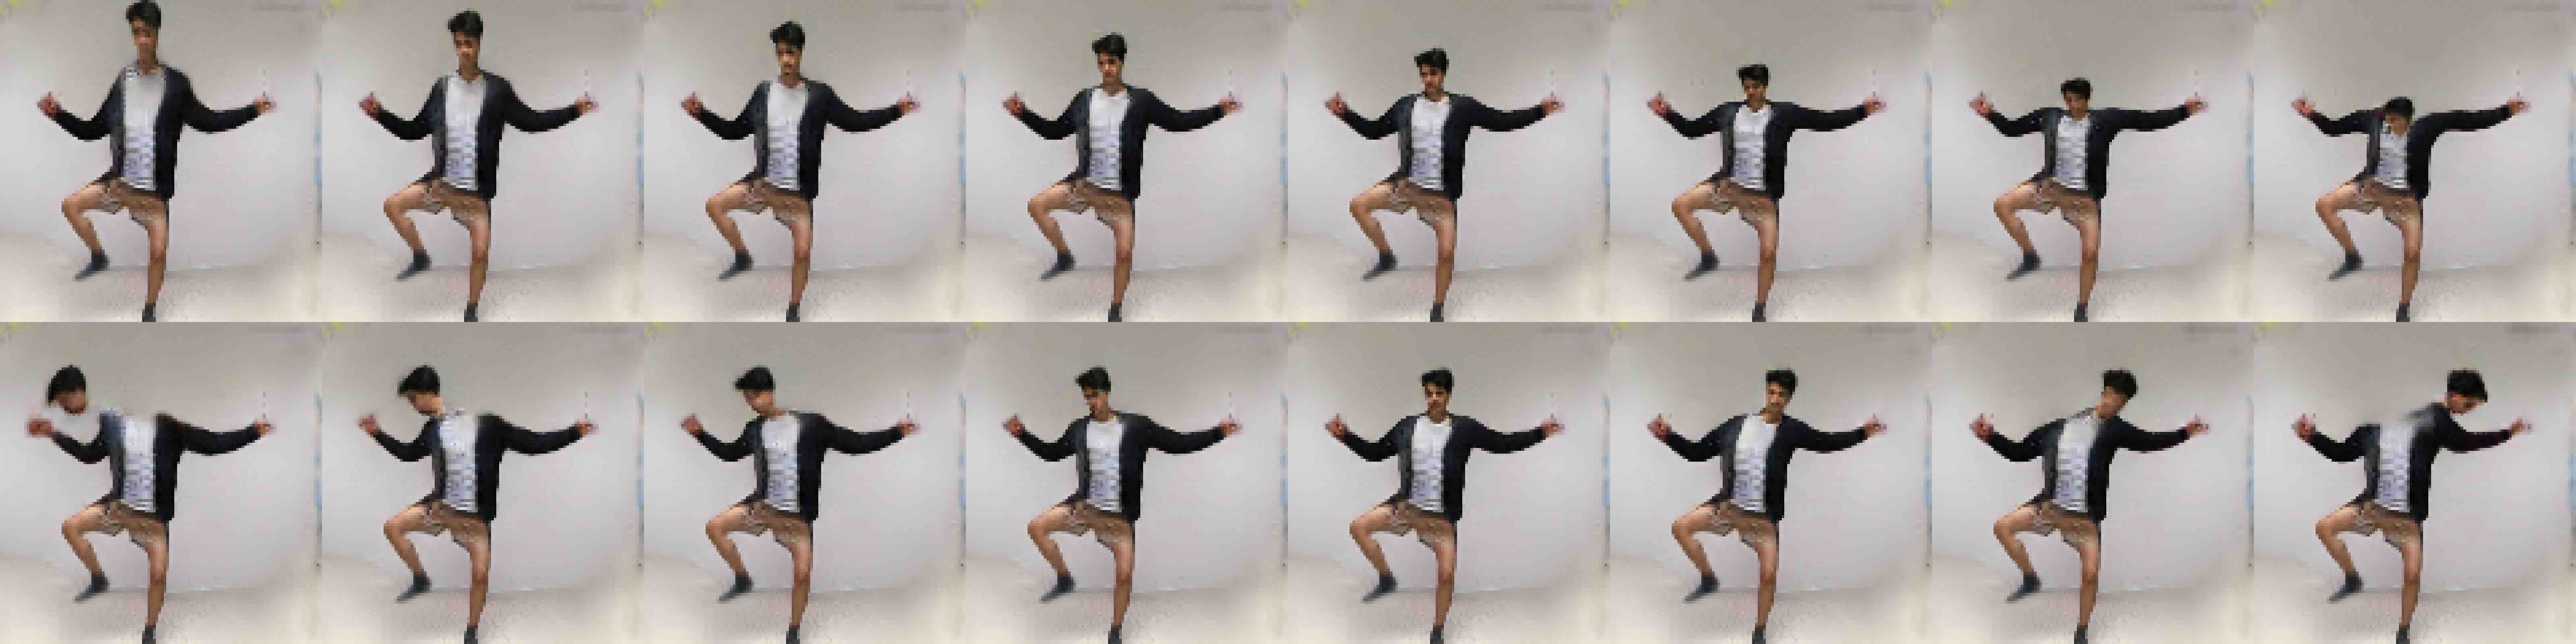
\includegraphics[trim={0cm 0cm 0cm 0cm},clip, width=1.0\linewidth]{fig/factor/8head}\caption{}
		\end{subfigure}
		\caption{Moving individual body landmarks for conditional generation: (a) arm (b) head.}
		\label{fig:movekp}
	\end{figure}

